\documentclass[class=report, crop=false, 12pt,a4paper]{standalone}
\usepackage{enumitem}
\usepackage{multicol}
\usepackage{etoolbox}
\AtBeginEnvironment{quote}{\singlespacing\small}
\usepackage{setspace}
\onehalfspacing
\usepackage{graphicx}
\usepackage{float}
\usepackage{amsmath}
\usepackage{amssymb}
\usepackage{siunitx}
\sisetup{detect-all}
\begin{document}
\section{Vapour and combined power cycles}
Vapour cycle:
\begin{itemize}[noitemsep]
  \item The working fluid exists in the vapour phase during one part of the cycle and in the liquid phase during another part.
  \item The liquid (working fluid) is alternatively vaporised and condensed.
\end{itemize}
Steam is the most common working fluid used in vapour power cycles:
\begin{itemize}[noitemsep]
  \item Low cost.
  \item Availability.
  \item High enthalpy of vaporisation.
\end{itemize}
\subsection{The Carnot vapour cycle}
The Carnot cycle is the most efficient cycle operating between two specified temperature levels - it is adopted as an ideal cycle. Steam is the working fluid in the Carnot vapour cycle. Below we contemplated why this cycle is not a suitable model for a power cycle. Consider a steady flow Carnot cycle is executed within the saturation dome of a pure substance as shown in Figure (\ref{CarnotVapourCycle}). 
\begin{itemize}[noitemsep]
  \item Process 1-2: reversible isothermal heat addition in a boiler. 
  \item Process 2-3: isentropic expansion in a turbine.
  \item Process 3-4: isothermal heat rejection (condensation occurs in a condenser).
  \item Process 4-1: isentropic compression in a compressor, to the initial state.
\end{itemize}
\begin{figure}
  \centering
  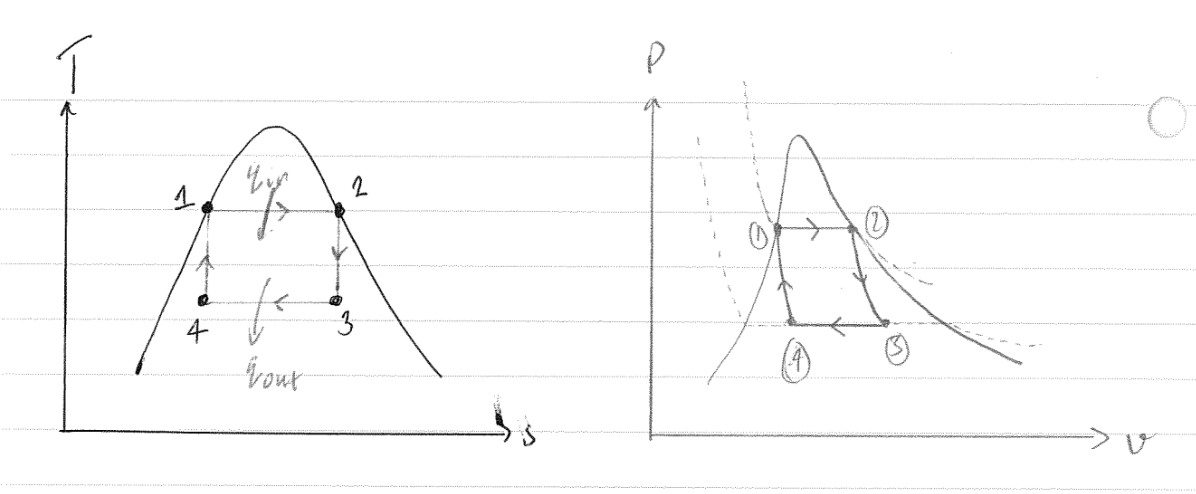
\includegraphics[width = 0.8 \textwidth]{../img/CarnotVapourCycleTSPV}
  \caption{Ts and Pv diagrams for the Carnot vapour cycle.}
  \label{CarnotVapourCycle}
\end{figure}
\subsection{Impracticalities of the Carnot vapour cycle}
\begin{enumerate}[noitemsep]
  \item Isothermal heat transfer to or from a two-phase system is not difficult to achieve in practice, since maintaining a constant pressure in the device automatically fixes the temperature at the saturation value. Thus, processes 1-2 and 3-4 can be approached closely by actual boilers and condensers. However, limiting the heat transfer process to two phase systems, severely limits the maximum temperature that can be used in the cycle as it has to remain under the critical point value (turning point) which is 374 \si{\celsius} for water. Limiting the maximum temperature leads to limiting the maximum efficiency. you could do a single phase heat transfer, but it is difficult to achieve this isothermally. 
  \item The isentropic expansion process (2-3) can be approximated closely by a well-designed turbine. However, the quality of the steam decreases during this process. Thus, the steam has a higher moisture content. Water droplets can cause erosion on turbine blades. Thus, steam with $x<90\% $ cannot be tolerated in the operation of power plants. This can be eliminated by using a working fluid with a very steep saturated vapour line.
  \item Process 3-4 is an isothermal heat rejection and condensation process. It is difficult to end up with the desired quality at state 4.
  \item Process 4-1 is an adiabatic, isentropic (reversible compression) process. However, it is not practical to design a compressor that handles two phases.
\end{enumerate}
Some of these problems can be eliminated by executing the carnot cycle as shown in Figure (\ref{BetterCarnot}).
\begin{figure}
  \centering
  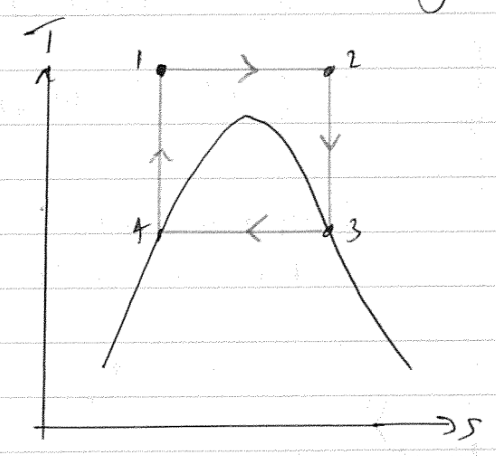
\includegraphics[width = 0.6 \textwidth]{../img/BetterCarnotTS}
  \caption{Ts diagram for an alternative Carnot vapour cycle.}
  \label{BetterCarnot}
\end{figure}
However, this cycle presents other problems such as isentropic compression to extremely high pressures and isothermal heat transfer at variable pressures. This cycle however presents other problems such as isentropic compression to extremely high pressures and isothermal heat transfer at variable pressures. Thus, we conclude that the Carnot cycle cannot by approximated in actual devices and is not a realistic model for vapour power cycles. 
\subsection{Rankine cycle: the ideal cycle for vapour power cycles}
The Rankine cycle is the ideal cycle to represent vapour power plants. It does not involve any internal irreversibilities and consists of the following four processes:
\begin{itemize}[noitemsep]
  \item Process 1-2: isentropic compression in a pump.
  \item Process 2-3: isobaric heat addition in a boiler.
  \item Process 3-4: isentropic expansion in a turbine.
  \item Process 4-1: isobaric heat rejection in a condenser.
\end{itemize}
\begin{figure}
  \centering
  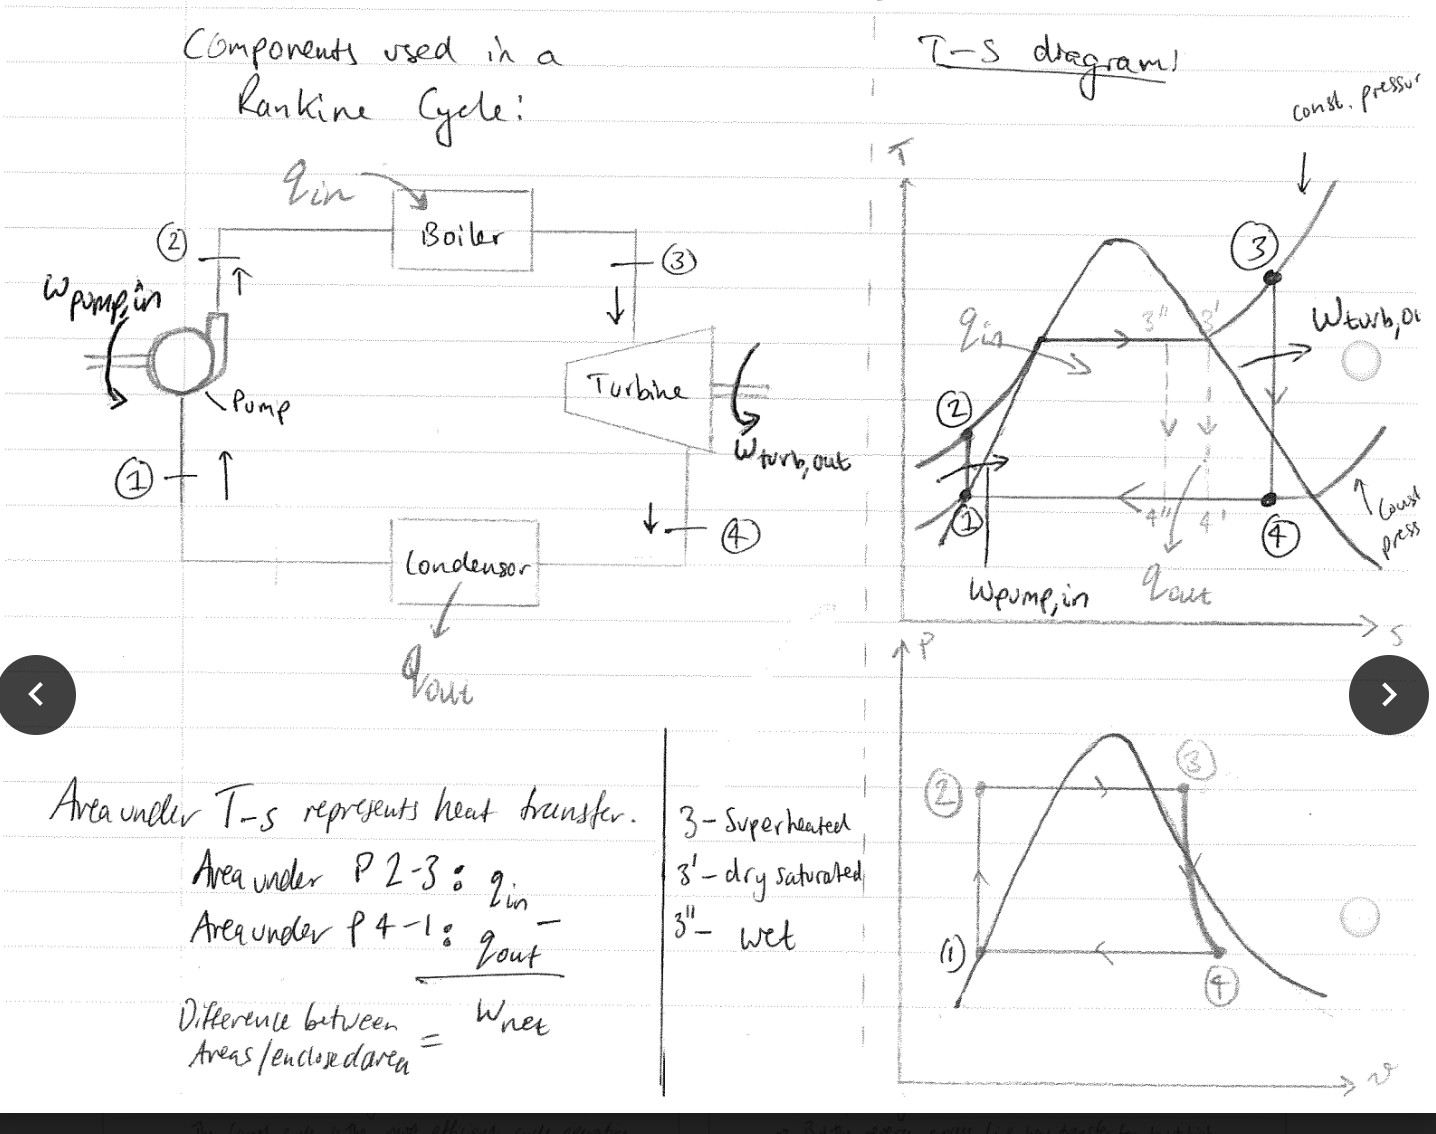
\includegraphics[width = 0.9\textwidth]{../img/RankineCycle}
  \caption{Component diagram and Ts Pv diagrams for the Rankine cycle.}
\end{figure}
\subsection{Qualitative description of the Rankine cycle}
\subsubsection{Water enters pump: state 1 to state 2}
Water enters pump at state 1 as a saturated liquid. Isentropic compression raises the pressure of the water to the boilers operating pressure. Temperature of water increases due to a slight decrease in the specific volume of water. Check entropy notes. Remember, during an isentropic process, for truly incompressible liquids and solids, temperature remains constant. Thus, if water was truly incompressible, there would not be a temperature rise during an isentropic compression process. Thus, on the Pv graph, the isentropic process is shown as a straight line, as v doesn't change, but pressure does, for incompressible substances. This diagram is the ideal one.
\subsubsection{Water enters boiler: state 2 to state 3}
Water is now a compressed liquid as it enters the boiler. The boiler exchanges heat into the liquid, causing it to evaporate, until it reaches state 3 and leaves as a superheated vapour. The heat exchange process occurs at constant pressure.
\subsubsection{Water enters turbine: state 3 to state 4}
Superheated vapour enters the turbine and expands isentropically and produces work. Pressure and temperature drop to that of state 4. Water is now a saturated liquid-vapour mixture with a high quality.
\subsubsection{Water enters the condenser: state 4 to state 1}
Saturated liquid-vapour mixture with high quality is condensed at constant pressure in a condenser. Heat is rejected for cooling medium, e.g. lake, atmospheric. Steam leaves the condenser as a saturated liquid and enters the pump, completing the cycle. Dry cooling, as used in cars or planes, where water is precious, is when heat is reject to air instead of water.
\subsection{Energy analysis of the ideal Rankine cycle}
All four components are steady flow devices. Neglect kinetic and potential energy changes as they are usually small relative to the work and heat transfer terms.
\subsubsection{SFEE per unit mass}
\begin{equation}
  \dot{Q}_{in} + \dot{W}_{in} + \dot{m}_1 h_1 = \dot{Q}_{out} + \dot{W}_{out} + \dot{m}_2 h_2
\end{equation}
$(\dot{m} = \dot{m}_1 = \dot{m}_2)$ and so dividing by $\dot{m}$ gives:
\begin{equation}
  q_{in} + w_{in} + h_1 = q_{out} + w_{out} + h_2
\end{equation}
Pump: 1-2 isentropic compression:
\begin{gather}
  q = 0,\  w_{out} = 0, \ w_{in} = w_{\textrm{pump in}}\\
  w_{\textrm{pump in}} = h_2 - h_1\\
  w_{\textrm{pump in}} = v(P_2 - P_1)
\end{gather}
Boiler: 2-3 isobaric heat addition
\begin{gather}
  w = 0,\  q_{out} = 0\\
  q_{in} = h_3 - h_2
\end{gather}
Turbine: 3-4 isentropic expansion:
\begin{gather}
  w = 0,\ q_{in} = 0\\
  q_{out} = h_4 - h_1\\
  \eta_{th, \ rankine} = \frac{w_{net}}{q_{in}} = 1 - \frac{q_{out}}{q_{in}} = \frac{w_T - w_P}{q_{in}}\\
  \eta_{th, \ rankine} = \frac{(h_3 - h_4) - (h_2 - h_1)}{h_3 - h_2}\\
  \eta_{th, \ rankine} = 1 - \frac{h_4 - h_1}{h_3 - h_2}
\end{gather}
The pump handles liquid (water) which is incompressible. Its density or v, specific volume, undergoes little change with increase in pressure.
\subsubsection{Using the Tds relations}
\begin{equation}
  Tds = dh - vdP
\end{equation}
For reversible adiabatic compression, $ds = 0$
\begin{align}
  Tds = 0 &= dh - vdP\\
  dh &= vdP\\
  \Delta h &= v\Delta P\\
  h_2 - h_1 &= v_1 (P_2 - P_1)\\
  \textrm{remember } w_{pump,\  in} &= h_2 - h_1 = v_1 (P_2 - P_1)
\end{align}
where $h_1 = h_{f@P_1}$ and $v_1 = v_{f@P_1}$.

Isentropic efficiencies:
\begin{align}
  \eta_T &= \frac{w_a}{w_s} = \frac{h_3 - h_{4a}}{h_3 - h_{4s}}\\
  \eta_P &= \frac{w_s}{w_a} = \frac{h_{2s} - h_{1}}{h_{2a} - h_{1}}
\end{align}
\end{document}